% CVPR 2026 Paper Template adapted for the DIP course project.

\documentclass[10pt,twocolumn,letterpaper]{article}

\usepackage[final]{cvpr}
\usepackage{amsmath}
\usepackage{amssymb}
\usepackage{booktabs}
\usepackage{multirow}
\usepackage{array}
\usepackage{graphicx}
\usepackage{xspace}
\usepackage{xcolor}

\definecolor{cvprblue}{rgb}{0.21,0.49,0.74}
\usepackage[pagebackref,breaklinks,colorlinks,allcolors=cvprblue]{hyperref}
\DeclareMathOperator*{\argmin}{arg\,min}
\DeclareMathOperator*{\argmax}{arg\,max}
\newcommand{\method}{PG-DSRNet\xspace}

\def\paperID{DIP26}
\def\confName{CVPR}
\def\confYear{2026}

\title{Prior-Guided DSRNet for Single Image Reflection Removal:\\
Reproduction, Lightweight Priors, and Real-World Analysis}

\author{TODO\_NAME (TODO\_ID)\\
Fudan University\\
{\tt\small TODO\_EMAIL}
}

\begin{document}
\maketitle

\begin{abstract}
Single image reflection removal aims to recover the clean transmission layer from a photograph captured through glass.
The task is severely ill-posed because the observed image can be explained by many transmission/reflection decompositions, and real reflections often share edges, textures, and color statistics with the background.
This course project first reproduces the required ERRNet baseline and compares it with DSRNet, a recent component-synergy model that jointly predicts transmission and reflection.
We then propose a lightweight prior-guided variant, \method, which keeps the DSRNet-L architecture and inference interface unchanged but adds two training-time losses: a low-/high-frequency transmission loss and a reflection-intensity weighted residual loss.
Experiments are conducted on CEILNet synthetic table2, Berkeley real20, SIR$^2$ Objects/Postcard/Wild, and five self-collected clean photographs with synthesized reflections.
The results are mixed but informative: \method improves CEILNet table2 by 0.866 dB PSNR over our reproduced DSRNet-L baseline, but it degrades on real20 and most SIR$^2$ subsets, revealing a domain gap between prior-guided fine-tuning and real reflection statistics.
We report these outcomes honestly and discuss when lightweight priors help and when they overfit synthetic cues.
\end{abstract}

\section{Introduction}

Photographs taken through glass are common in daily life: shop windows, train windows, museum showcases, and night scenes often contain a superposition of the desired scene and reflected content.
Single image reflection removal (SIRR) attempts to recover the clean transmission layer from one contaminated image.
A widely used image formation model writes
\begin{equation}
    I = T + R * h + \epsilon,
    \label{eq:image_formation}
\end{equation}
where $I$ is the observed image, $T$ is the desired transmission layer, $R$ is the reflection layer, $h$ denotes blur or ghosting, and $\epsilon$ absorbs sensor noise and saturation.
With only one input image, this inverse problem is under-constrained: many pairs $(T,R)$ can explain the same $I$.
The difficulty is amplified in real scenes because reflection edges can be as sharp as background edges, glass may introduce spatially varying attenuation, and real paired training images are often imperfectly aligned.

The course requirement asks for a deep-learning baseline, an improved method, quantitative comparisons using PSNR, SSIM, NCC, and LMSE, and visual analysis on both public benchmarks and five self-collected photographs.
We choose ERRNet~\cite{wei2019errnet} as the required baseline because it explicitly targets misaligned real training data and is the official course baseline.
For the improved method, we reproduce DSRNet~\cite{hu2023dsrnet}, which models transmission, reflection, and reconstruction jointly through component synergy.
To add a project-level modification, we further introduce \method, a lightweight training-only extension of DSRNet-L inspired by recent prior-guided restoration work.

\method is intentionally conservative.
It does not add a diffusion model, transformer backbone, user mask, or extra inference input.
Instead, it adds two losses during fine-tuning.
First, a frequency loss supervises both low-frequency color/illumination and high-frequency structural residuals of the predicted transmission.
Second, a reflection-prior loss weights residual supervision in regions where a reflection-intensity prior and input high-frequency response indicate stronger reflection interference.
This design is motivated by PromptRR-style frequency guidance~\cite{wang2024promptrr} and FUMO-style prior/high-frequency modulation~\cite{desmon2024fumo}, while staying comparable to the automatic ERRNet/DSRNet setting.

Our main finding is not a simple win.
Under the unified evaluator, reproduced DSRNet-L is stronger than reproduced ERRNet on CEILNet table2, Objects, Postcard, and Wild, but ERRNet remains stronger on real20.
\method improves CEILNet table2 but usually reduces performance on real benchmarks.
On five self-collected clean images with synthesized reflections, ERRNet performs best under our synthesis protocol, while \method only slightly improves over DSRNet-L.
These results suggest that lightweight priors can strengthen synthetic-data reconstruction but require more robust real-data calibration.

\section{Related Work}

\paragraph{Traditional layer separation.}
Early reflection removal methods formulate the task as image layer separation and impose hand-crafted priors on gradients, edges, or smoothness.
Levin and Weiss~\cite{levin2007user} studied user-assisted separation, while Li and Brown~\cite{li2014single} modeled reflection separation through gradient statistics and optimization.
These methods are interpretable and do not require large training sets, but they struggle when the reflection has strong edges, repeated textures, or spatially varying blur.

\paragraph{CNN and perceptual learning.}
Deep models moved SIRR from hand-crafted optimization to learned restoration.
CEILNet and related early CNN methods~\cite{fan2017generic} learn a direct mapping from reflection-contaminated images to clean transmission images, improving synthetic benchmark performance.
Zhang et al.~\cite{zhang2018perceptual} introduced perceptual losses and real paired data, showing that feature-level supervision can better preserve visual realism than pure pixel losses.
However, real paired reflection data are small and often misaligned, so models trained on synthetic data may still fail on real glass scenes.

\paragraph{Misaligned real-data learning.}
ERRNet~\cite{wei2019errnet} is the required course baseline.
It uses VGG hypercolumn features, channel-wise context, and multi-scale spatial context to improve restoration, and it introduces losses that can exploit misaligned real-world pairs.
This makes ERRNet a strong and practical baseline for the course setting: it is compact enough to train, supports the required datasets, and reports PSNR, SSIM, NCC, and LMSE.

\paragraph{Component-synergy and refinement models.}
Later work explores stronger decomposition consistency.
IBCLN~\cite{li2020ibcln} refines transmission and reflection through a cascaded bidirectional architecture.
DSRNet~\cite{hu2023dsrnet} jointly predicts transmission, reflection, and reconstructed mixture, using component synergy to make the separated layers mutually constrained.
This explicit decomposition is attractive for analysis because it yields both transmission and reflection outputs, but it remains supervised and sensitive to data protocol details.

\paragraph{Recent priors, prompts, and benchmarks.}
Prompt-based and diffusion-style reflection removal methods seek stronger priors for difficult real cases.
PromptRR~\cite{wang2024promptrr} emphasizes low-/high-frequency information and prompt-guided restoration.
FUMO~\cite{desmon2024fumo} uses intensity and high-frequency priors to modulate restoration.
FIRM~\cite{chen2025firm} studies user- or mask-guided reflection removal, which is powerful but changes the task from fully automatic SIRR to interactive restoration.
Recent benchmark work such as OpenRR-5k~\cite{cai2025openrr} argues that older real benchmarks are too small and that no-reference or large-scale real evaluations are needed.
In this project, these recent directions motivate our lightweight prior losses and our discussion of limitations, but we do not introduce diffusion models, user masks, or new large-scale training data.

\section{Method}

\subsection{Baseline: ERRNet}
ERRNet~\cite{wei2019errnet} takes a reflection-contaminated image as input and predicts the transmission layer.
Its backbone contains residual blocks augmented by VGG hypercolumn features.
A channel-wise context module reweights global feature responses, and a pyramid pooling module provides multi-scale spatial context.
During training, ERRNet combines reconstruction and perceptual supervision and supports an alignment-invariant loss for misaligned real pairs.
We use both the released ERRNet checkpoint for official-protocol reference and our reproduced/fine-tuned checkpoint for the self-trained comparison.

\subsection{Improved Baseline: DSRNet}
DSRNet~\cite{hu2023dsrnet} predicts a transmission layer $\hat{T}$, a reflection layer $\hat{R}$, and a reconstructed mixture.
Instead of treating reflection removal as only image-to-image translation, it enforces consistency among the separated components.
For our main reproduction, we train DSRNet-L under Setting I with VGG and reconstruction losses and evaluate it with the same wrapper/evaluator as ERRNet.

\subsection{Proposed Prior-Guided DSRNet}
The proposed \method keeps the DSRNet-L architecture and inference interface unchanged.
Only the training objective is modified:
\begin{equation}
    \mathcal{L}
    =
    \mathcal{L}_{\mathrm{DSR}}
    +
    \lambda_{\mathrm{freq}}\mathcal{L}_{\mathrm{freq}}
    +
    \lambda_{\mathrm{prior}}\mathcal{L}_{\mathrm{prior}} .
    \label{eq:total_loss}
\end{equation}
This makes the method easy to compare with DSRNet because no extra test-time prompt, mask, or model component is required.
Figure~\ref{fig:pipeline} illustrates the training flow.

\begin{figure*}[t]
    \centering
    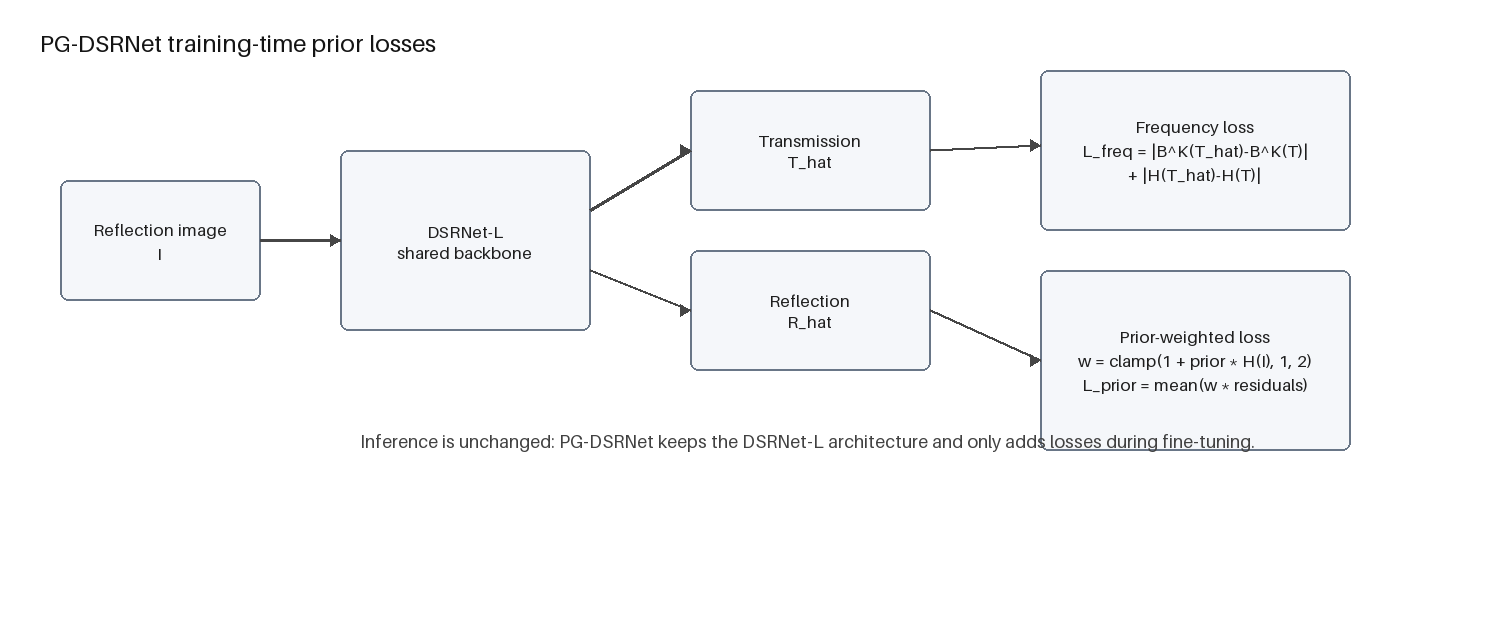
\includegraphics[width=0.95\linewidth]{figures/fig_method_pipeline.png}
    \caption{Overview of \method. The DSRNet-L architecture is unchanged. We add a frequency loss on the predicted transmission and a reflection-prior weighted residual loss during fine-tuning.}
    \label{fig:pipeline}
\end{figure*}

\paragraph{Frequency loss.}
Let $B(\cdot)$ be a fixed depthwise blur operator, and let $B^K$ denote applying it for $K$ levels.
We define the high-frequency residual as
\begin{equation}
    H(X) = X - B^K(X).
\end{equation}
The frequency loss supervises both color/illumination structure and high-frequency details:
\begin{equation}
    \mathcal{L}_{\mathrm{freq}}
    =
    \|B^K(\hat{T}) - B^K(T)\|_1
    +
    \|H(\hat{T}) - H(T)\|_1 .
    \label{eq:freq_loss}
\end{equation}
This is a lightweight substitute for prompt-based frequency modeling: it does not learn prompts, but it directly penalizes errors in coarse and residual bands.

\paragraph{Reflection-prior weighted loss.}
For synthetic or paired data, a reflection prior can be estimated from the target reflection layer:
\begin{equation}
    P = \mathrm{norm}\left(\mathrm{mean}_c(|R|)\right).
\end{equation}
We combine this prior with the input high-frequency magnitude to form a spatial weight:
\begin{equation}
    W =
    \mathrm{clamp}\left(1 + P \odot \mathrm{mean}_c(|H(I)|), 1, 2\right).
    \label{eq:prior_weight}
\end{equation}
The weighted residual loss is
\begin{equation}
    \mathcal{L}_{\mathrm{prior}}
    =
    \mathrm{mean}\left[
    W \odot
    \left(
    |\hat{T}-T| + |\hat{R}-R|
    \right)
    \right].
    \label{eq:prior_loss}
\end{equation}
The intuition is simple: reflection-heavy and structure-sensitive regions should receive stronger supervision.
In our experiments we fine-tune from the reproduced DSRNet-L checkpoint with $\lambda_{\mathrm{freq}}=0.05$ and $\lambda_{\mathrm{prior}}=0.10$.

\section{Experiments}

\subsection{Datasets and Metrics}
We evaluate on the required benchmark family: CEILNet synthetic table2, Berkeley/Zhang real20, and the SIR$^2$ Objects, Postcard, and Wild subsets.
For the self-collected part, we use five clean photographs in the project folder \texttt{self/} as transmission ground truth and synthesize reflection-contaminated inputs with a fixed seed.
The synthesis uses a real-image source as reflection, Gaussian blur, a smooth spatial mask, and the formula
$M=\mathrm{clip}(\alpha_t T+\alpha_r B(R)\odot mask,0,1)$.
This gives full-reference metrics for the five custom images while keeping the process reproducible.

We report PSNR, SSIM, normalized cross-correlation (NCC), and local mean squared error (LMSE).
For PSNR, SSIM, and NCC, higher is better; for LMSE, lower is better.
The complete tables are exported in \texttt{paper/experiment\_results.md}; this section shows the main paper-facing results.

\subsection{Implementation Details}
ERRNet is trained with the official course branch and then fine-tuned on the real unaligned training set.
DSRNet-L is trained under Setting I with \texttt{--lambda\_vgg 0.01 --lambda\_rec 0.2 --if\_align --seed 2018}.
\method starts from this reproduced DSRNet-L checkpoint and fine-tunes with $\lambda_{\mathrm{freq}}=0.05$ and $\lambda_{\mathrm{prior}}=0.10$.
The frequency-only and prior-only ablations are trained to epoch55, while the combined \method run is trained to epoch60; therefore the ablation is informative but not a strict same-epoch controlled experiment.

\subsection{Horizontal Comparison}

\begin{table*}[t]
\centering
\small
\caption{Horizontal comparison on the five required public test sets under the unified evaluator. Each cell reports PSNR / SSIM. Official rows use released checkpoints, while reproduced rows use our trained checkpoints. The best PSNR in each dataset column is bolded.}
\label{tab:main_results}
\begin{tabular}{lccccc}
\toprule
Method & CEILNet & real20 & Objects & Postcard & Wild \\
\midrule
ERRNet official & 27.586 / 0.940 & \textbf{23.069 / 0.816} & 24.774 / 0.899 & 21.859 / 0.876 & 24.885 / 0.882 \\
DSRNet-L official epoch18 & 25.444 / 0.920 & 22.515 / 0.779 & \textbf{26.285 / 0.922} & \textbf{24.724 / 0.912} & 25.809 / 0.918 \\
ERRNet reproduced & 27.173 / 0.938 & 22.642 / 0.799 & 24.837 / 0.897 & 20.560 / 0.838 & 23.456 / 0.872 \\
DSRNet-L reproduced & \textbf{28.342 / 0.948} & 22.222 / 0.790 & 25.679 / 0.912 & 21.477 / 0.905 & \textbf{25.857 / 0.916} \\
\bottomrule
\end{tabular}
\end{table*}

Table~\ref{tab:main_results} separates released checkpoints from our self-trained checkpoints.
The released DSRNet-L epoch18 checkpoint is strongest on Objects and Postcard, while reproduced DSRNet-L is strongest on CEILNet and Wild.
ERRNet official remains strongest on real20 under the unified evaluator, which is consistent with the earlier observation that real20 is sensitive to resize and alignment protocol.

\subsection{Ablation Study}

\begin{table*}[t]
\centering
\small
\caption{\method ablation on the unified benchmark. Each cell reports PSNR / SSIM. The best PSNR in each dataset column is bolded. The combined frequency+prior run is trained to epoch60, while the single-loss runs are trained to epoch55.}
\label{tab:ablation}
\begin{tabular}{lccccc}
\toprule
Variant & CEILNet & real20 & Objects & Postcard & Wild \\
\midrule
DSRNet-L reproduced & 28.342 / 0.948 & \textbf{22.222 / 0.790} & \textbf{25.679 / 0.912} & \textbf{21.477 / 0.905} & \textbf{25.857 / 0.916} \\
+ frequency loss & 29.080 / 0.954 & 21.320 / 0.777 & 24.490 / 0.897 & 20.030 / 0.896 & 25.256 / 0.917 \\
+ prior loss & 29.002 / 0.954 & 21.506 / 0.780 & 24.593 / 0.899 & 20.101 / 0.898 & 25.474 / 0.919 \\
+ frequency + prior (\method) & \textbf{29.208 / 0.955} & 21.369 / 0.773 & 24.546 / 0.899 & 20.801 / 0.904 & 25.473 / 0.918 \\
\bottomrule
\end{tabular}
\end{table*}

Table~\ref{tab:ablation} shows that the proposed losses mainly improve CEILNet synthetic data.
The combined \method reaches 29.208 dB PSNR on CEILNet, a 0.866 dB gain over reproduced DSRNet-L.
However, the original reproduced DSRNet-L checkpoint remains best on real20 and all SIR$^2$ subsets.
This supports the interpretation that the frequency and reflection-intensity priors overfit synthetic reflection cues and do not yet generalize reliably to real reflection statistics.

\begin{table}[t]
\centering
\small
\caption{Self-collected synthetic reflection results on five clean custom photos.}
\label{tab:self_synth}
\begin{tabular}{lcccc}
\toprule
Method & PSNR & SSIM & NCC & LMSE \\
\midrule
ERRNet reproduced & \textbf{23.979} & \textbf{0.9616} & \textbf{0.9847} & \textbf{0.00163} \\
DSRNet-L reproduced & 14.040 & 0.3928 & 0.7256 & 0.08835 \\
\method & 14.066 & 0.3929 & 0.7288 & 0.08685 \\
\bottomrule
\end{tabular}
\end{table}

Table~\ref{tab:self_synth} reports the five-image self-collected synthetic set.
ERRNet performs best under this synthesis pipeline.
\method slightly improves over DSRNet-L, but the large gap to ERRNet shows that DSRNet-style models are sensitive to this custom synthesis distribution.

\begin{figure*}[t]
    \centering
    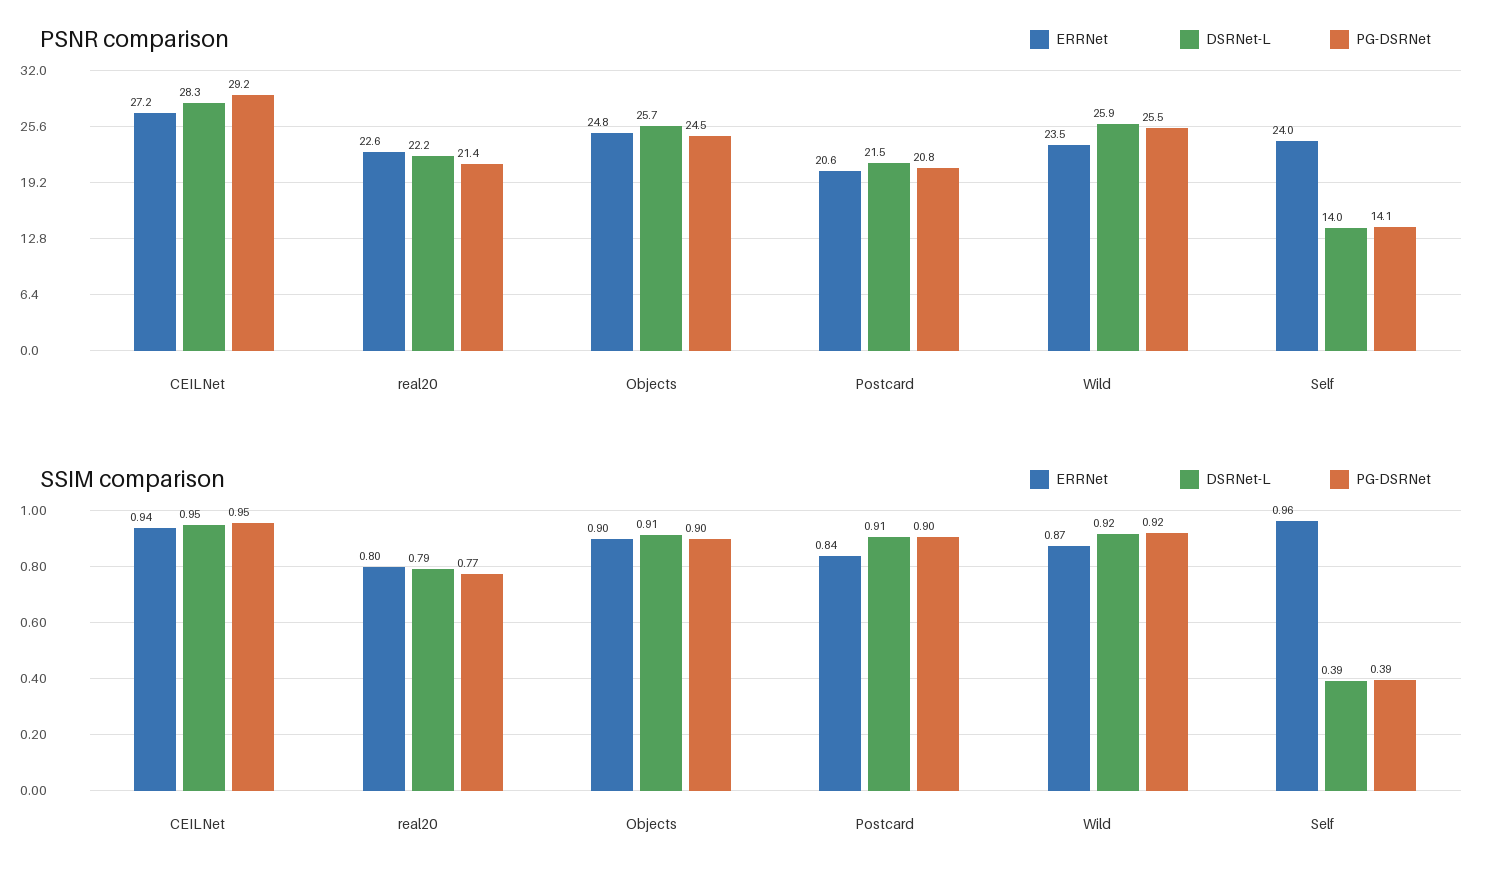
\includegraphics[width=0.95\linewidth]{figures/fig_quant_psnr_ssim.png}
    \caption{PSNR and SSIM visualization across public benchmarks and the self-collected synthetic set.}
    \label{fig:quant}
\end{figure*}

\begin{figure}[t]
    \centering
    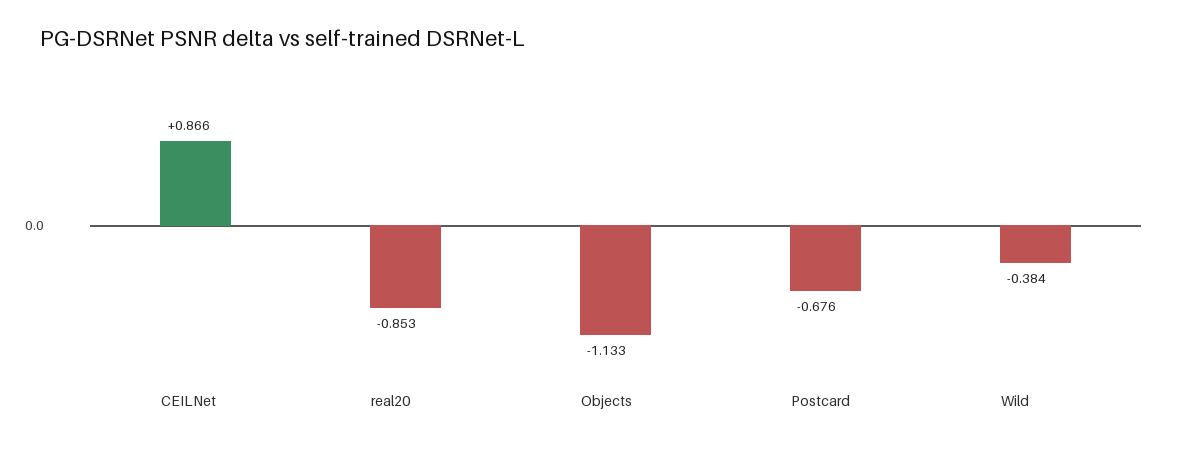
\includegraphics[width=\linewidth]{figures/fig_pg_delta.png}
    \caption{PSNR delta of \method relative to reproduced DSRNet-L. Positive values mean improvement.}
    \label{fig:delta}
\end{figure}

\subsection{Qualitative Results}
Figure~\ref{fig:qual_benchmark} shows representative public benchmark cases.
The DSRNet family often preserves cleaner structure on CEILNet and SIR$^2$, but the real20 example remains difficult.
Figure~\ref{fig:qual_custom} shows the five self-collected synthetic examples and confirms the quantitative trend: ERRNet removes the synthetic overlay more reliably in this particular custom synthesis protocol.

\begin{figure*}[t]
    \centering
    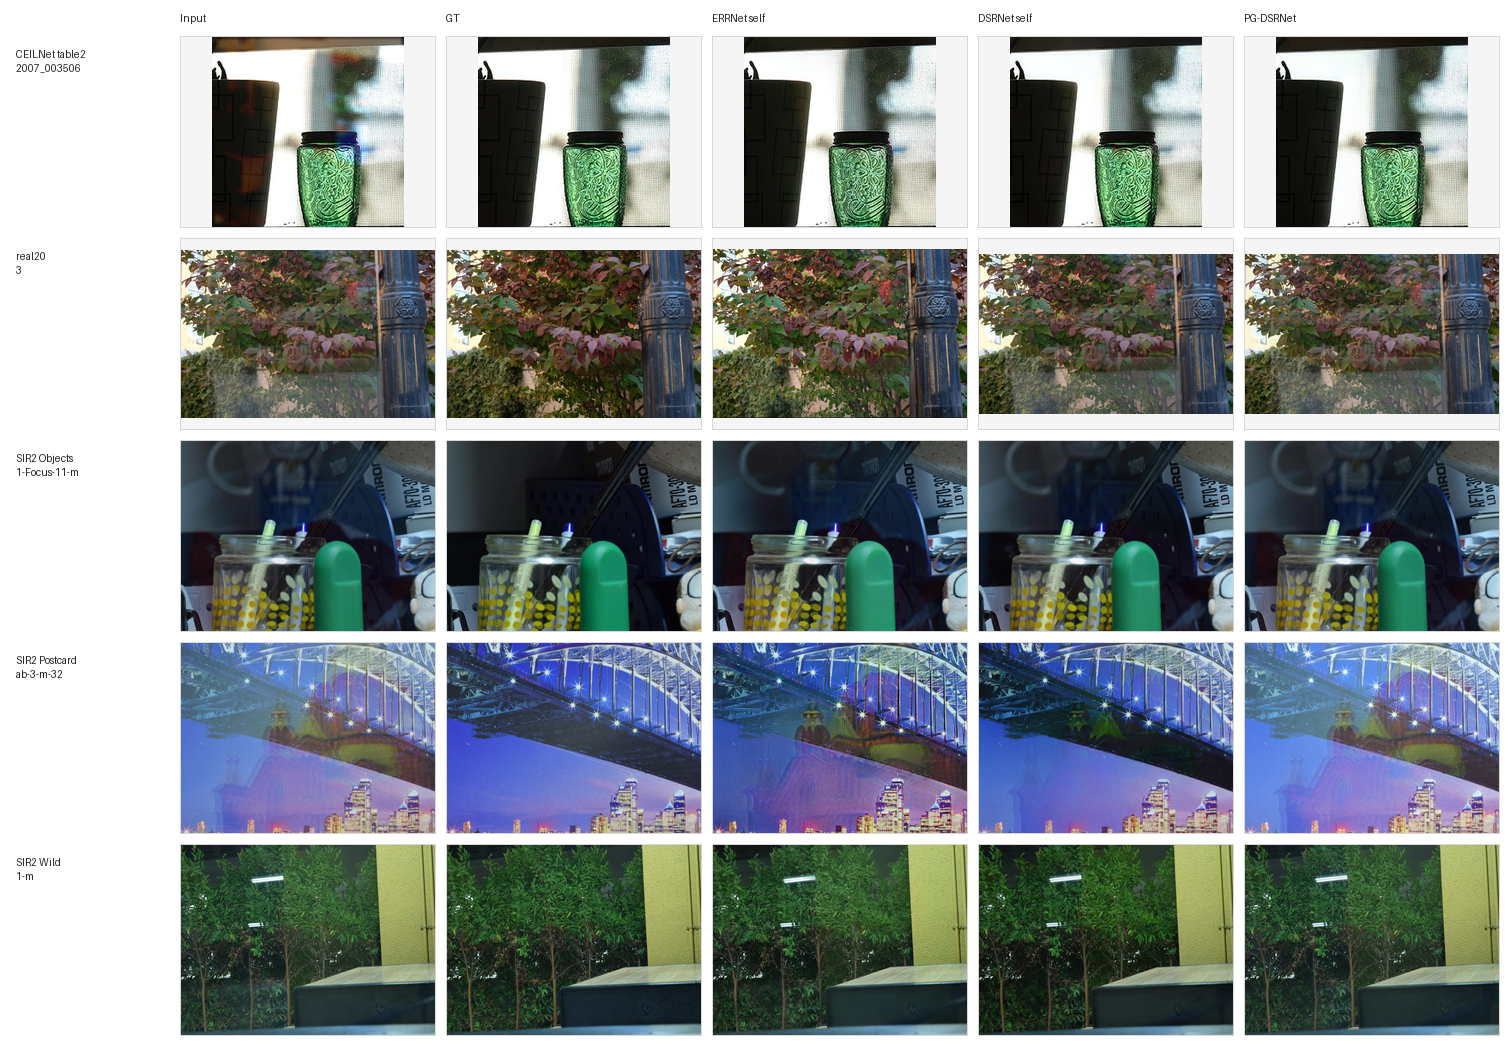
\includegraphics[width=0.98\linewidth]{figures/fig_qual_benchmark.png}
    \caption{Qualitative comparison on public benchmarks. Columns are input, ground truth, reproduced ERRNet, reproduced DSRNet-L, and \method.}
    \label{fig:qual_benchmark}
\end{figure*}

\begin{figure*}[t]
    \centering
    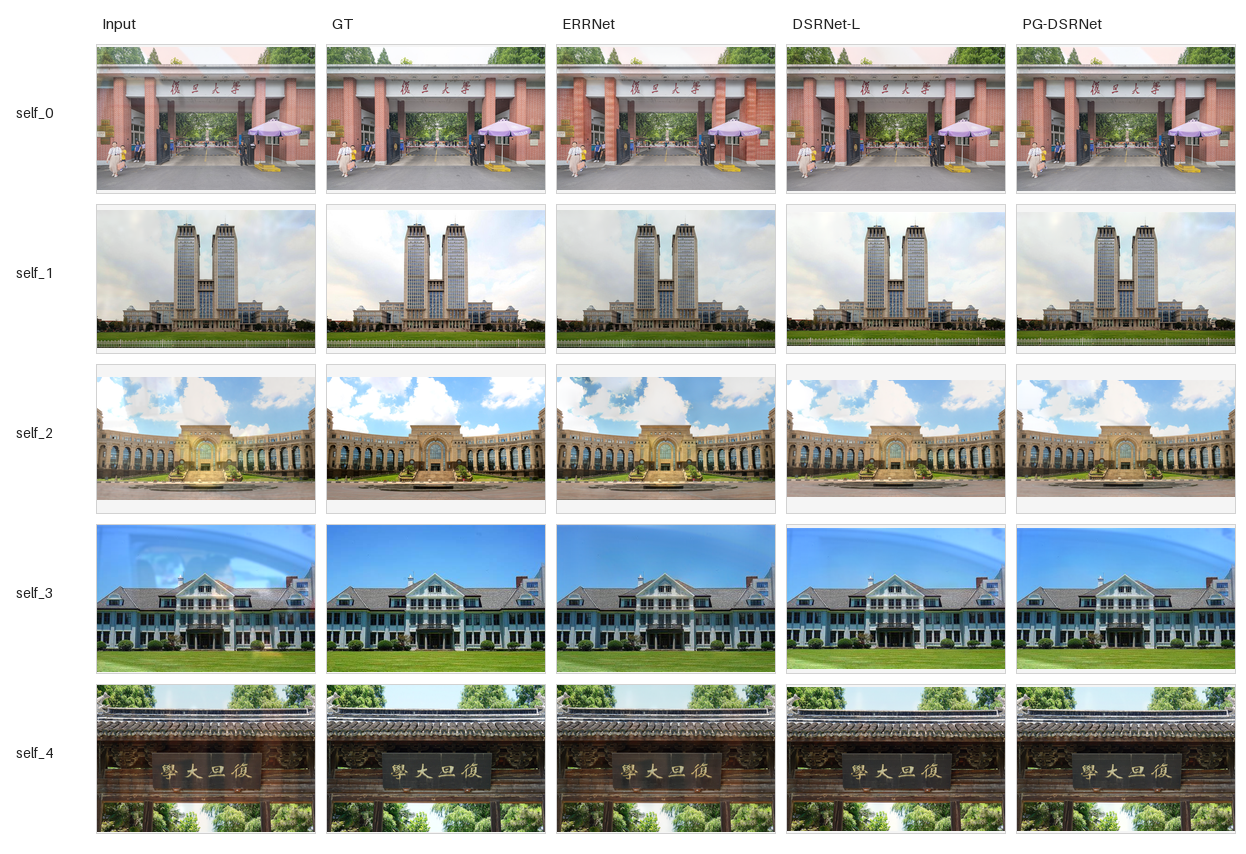
\includegraphics[width=0.98\linewidth]{figures/fig_qual_custom_synth.png}
    \caption{Qualitative comparison on five self-collected clean photos with synthesized reflections.}
    \label{fig:qual_custom}
\end{figure*}

\section{Discussion}

\paragraph{Why does \method help CEILNet but hurt real sets?}
The added losses emphasize frequency residuals and reflection-prior weighted regions.
On CEILNet synthetic images, the reflection generation process is closer to the assumptions of blur, additive reflection, and separable high-frequency residuals, so the priors provide useful extra supervision.
On real20 and SIR$^2$, the reflection may involve non-linear glass effects, saturation, ghosting, strong real edges, and imperfect alignment.
The same priors can then overweight ambiguous regions and push the model away from the real transmission layer.

\paragraph{Official protocol versus unified protocol.}
We keep official-protocol reproduction and unified-protocol comparison separate.
Under the DSRNet native protocol and official all-in-one data, DSRNet-L epoch18 reaches 23.882 dB PSNR on \texttt{real20\_420}, exceeding the local ERRNet native real20 PSNR of 23.553.
Under our unified evaluator on the course processed real20 split, ERRNet remains ahead of DSRNet-L.
This difference is not a contradiction; it reflects different resizing, alignment, and dataset-layout protocols.

\paragraph{Self-collected synthetic images.}
The five self-collected photos are clean images, so we synthesize reflections to obtain ground truth metrics.
This satisfies full-reference evaluation, but it also introduces a new synthetic distribution.
The poor DSRNet-L and \method scores on this set suggest that the synthesis pipeline is closer to the ERRNet training/evaluation assumptions than to the DSRNet Setting I data distribution.
For real deployment, a larger real dataset with paired or carefully captured reference images would be more reliable.

\paragraph{Limitations.}
The current \method is a lightweight loss-only modification, so its innovation is modest compared with large prompt or diffusion models.
It is also fine-tuned from a reproduced DSRNet-L checkpoint instead of being trained from scratch under a fully controlled schedule.
Finally, the combined loss run uses more epochs than the single-loss ablations, so the ablation should be interpreted as completed experimental evidence rather than strict causal proof.
Future work could add same-epoch controls, stronger real-data priors, or an interactive mask-guided branch inspired by FIRM, while keeping the automatic benchmark setting clearly separated.

\section{Conclusion}

This project reproduces the required ERRNet baseline, trains and evaluates DSRNet-L as an improved component-synergy method, and proposes \method as a lightweight prior-guided fine-tuning variant.
The experiments show that DSRNet-L is generally stronger than ERRNet on several public subsets, while ERRNet remains competitive and even superior on real20 and the self-collected synthetic set.
\method improves CEILNet table2 but does not generalize consistently to real benchmarks, highlighting the central challenge of reflection removal: synthetic priors are useful, but real glass reflections are more diverse than the simplified formation model.

The submitted repository contains the training/evaluation code, reproducible result summaries, paper figures, and documentation for separately uploaded weights.
The GitHub repository is available at \href{https://github.com/MarshCurrant/PG_DSRNet}{MarshCurrant/PG\_DSRNet}.
The model weights are shared via Baidu Netdisk: \href{https://pan.baidu.com/s/151h3CPe1i1OpOMrLGYMfKA?pwd=1234}{DIP} (extraction code: 1234).
Member contribution: TODO\_CONTRIBUTION.

\appendix
\section{AI Assistance Statement}

OpenAI Codex was used as an AI assistant during this course project.
Its assistance covered three main aspects.
First, Codex helped read and organize the literature survey by summarizing reflection-removal methods, comparing ERRNet, DSRNet, PromptRR, FUMO, FIRM, and OpenRR-5k, and turning the survey notes into a structured related-work outline.
Second, Codex helped build and debug the experimental pipeline, including dataset layout checks, inference wrappers, benchmark aggregation scripts, self-collected synthetic reflection generation, qualitative figure generation, and Markdown/LaTeX result tables.
Third, Codex helped polish the paper language, improve LaTeX formatting, and refine the presentation of negative and mixed experimental findings.

All model choices, experiment execution, result verification, and final interpretations were checked by the author.
The quantitative numbers reported in this paper come from local benchmark scripts, saved logs, and generated summary files rather than from AI generation.
Codex was therefore used as a research, coding, and writing assistant, while the responsibility for correctness, academic integrity, and final claims remains with the author.

{
    \small
    \bibliographystyle{ieeenat_fullname}
    \bibliography{main}
}
\end{document}
